%----------------------------------------------------------------------------------------
%	PACKAGES AND THEMES
%----------------------------------------------------------------------------------------
\documentclass[aspectratio=169,xcolor=dvipsnames]{beamer}
\usetheme{Simple}

\usepackage{hyperref}
\usepackage{MnSymbol}
\usepackage{graphicx} % Allows including images
\usepackage{booktabs} % Allows the use of \toprule, \midrule and \bottomrule in tables

%----------------------------------------------------------------------------------------
%	TITLE PAGE
%----------------------------------------------------------------------------------------

% The title
\title[short title]{LANTSA: Landmark-based transferable subspace analysis for
single-cell and spatial transcriptomics}
\subtitle{}

\author[Pin-Yen] {Reporter: Musu Yuan}
\institute[NTU] % Your institution may be shorthand to save space
{
    % Your institution for the title page
    CQB, AAIS, Peking University, Beijing
    \vskip 3pt
}
\date{December $5^{th}$, 2021} % Date, can be changed to a custom date


%----------------------------------------------------------------------------------------
%	PRESENTATION SLIDES
%----------------------------------------------------------------------------------------

\begin{document}

\begin{frame}
\begin{figure}
    \centering
    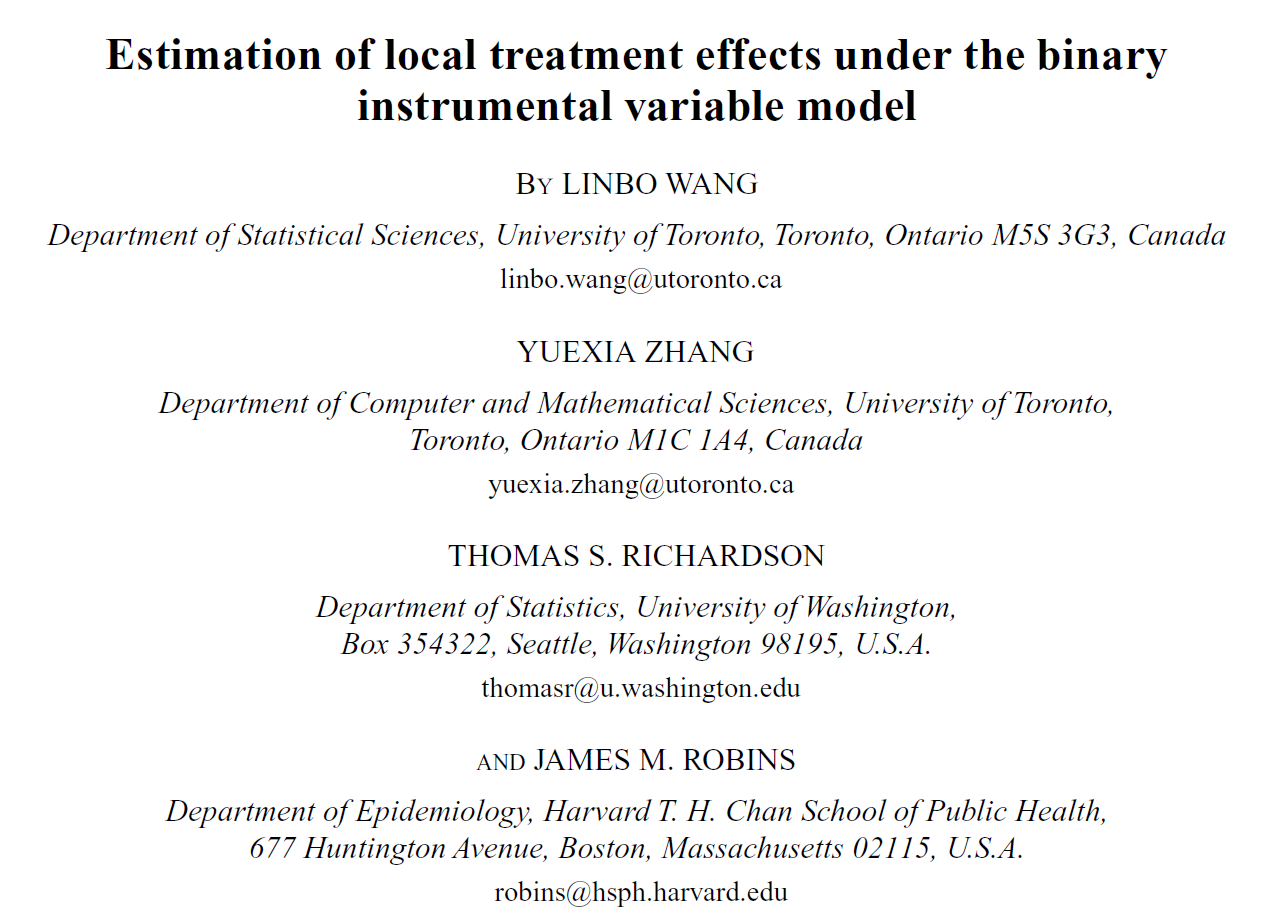
\includegraphics[width=0.7\textwidth]{figure/fig1.PNG}
\end{figure}
\end{frame}

\begin{frame}{Background}
Unmeasured confounding occurs in observational studies as well as imperfect randomized controlled trials.\vspace{8pt}\\
An instrumental variable is a pre-treatment covariate that is associated with the outcome only through its effect on the treatment.
\end{frame}

\begin{frame}{Instrumental Variable methods}
  \begin{itemize}
      \item average treatment effect\\ \quad relies on untestable homogeneity assumptions involving unmeasured confounders\vspace{8pt}
      \item local average treatment effect\\ \quad can be nonparametrically identified under a certain monotonicity
assumption
  \end{itemize} 
\end{frame}

\begin{frame}{Framework}
\textbf{Causal effect estimation with a binary exposure indicator D and a binary outcome Y} \vspace{8pt}\\
Suppose that the effect of D on Y is subject to confounding by observed variables X as well as unobserved variables U.\\
\begin{figure}
    \centering
    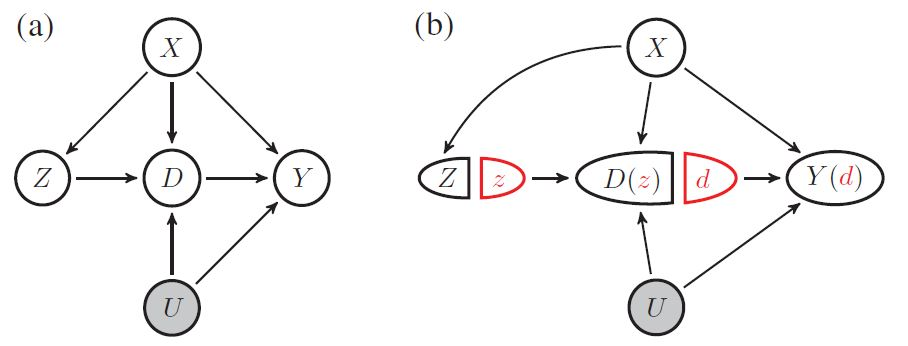
\includegraphics[width=0.7\textwidth]{figure/fig2.JPG}
\end{figure}
\end{frame}

\begin{frame}{Assumptions for Z}
\begin{itemize}
    \item (Exclusion restriction). For all $z$ and $z^{\prime}, Y(z, d)=Y\left(z^{\prime}, d\right) \equiv Y(d)$ almost surely.
\item (Independence). We have that $Z \upmodels (Y(d), D(z)) \mid X, d=0,1, z=0,1$.
\item (Instrumental variable relevance). We have that $\operatorname{pr}\{D(1)=1 \mid X\} \neq \operatorname{pr}\{D(0)=$ $1 \mid X\}$ almost surely.
\item (Positivity). There exists $\sigma>0$ such that $\sigma<\operatorname{pr}(Z=1 \mid X)<1-\sigma$ almost surely.
\item (Monotonicity). We have that $D(1) \geqslant D(0)$ almost surely.
\end{itemize}
\end{frame}

\begin{frame}{Principal strata}
\begin{figure}
    \centering
    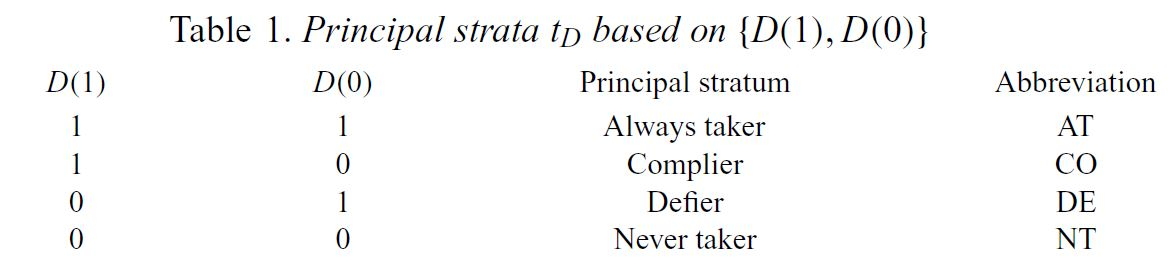
\includegraphics[width=0.8\textwidth]{figure/fig3.JPG}
\end{figure}
\end{frame}

\begin{frame}{Target}
We are interested in estimating the conditional treatment effects in the complier stratum on the additive and multiplicative scales\\
$$
\begin{aligned}
\operatorname{LATE}(X) &=E\{Y(1)-Y(0) \mid D(1)>D(0), X\}, \\
\operatorname{MLATE}(X) &=E\{Y(1) \mid D(1)>D(0), X\} / E\{Y(0) \mid D(1)>D(0), X\} .
\end{aligned}
$$
Abadie (2002, Lemma 2.1) showed that under Assumptions 1-5, the local average treatment effects are identifiable as
$$
\begin{aligned}
\operatorname{LATE}(X)&=\delta^{\mathrm{L}}(X) - \frac{E(Y \mid Z=1, X)-E(Y \mid Z=0, X)}{E(D \mid Z=1, X)-E(D \mid Z=0, X)},\\
\operatorname{MLATE}(X)&=\delta^{\mathrm{M}}(X) - \frac{E(Y D \mid Z=1, X)-E(Y D \mid Z=0, X)}{E\{Y(1-D) \mid Z=1, X\}-E\{Y(1-D) \mid Z=0, X\}}.
\end{aligned}
$$
\end{frame}

\begin{frame}{Frölich (2007)}
Define the conditional mean functions $m_{z}(x)=\mathrm{E}[Y \mid X=x, Z=z]$ and $\mu_{z}(x)=\mathrm{E}[D \mid X=x, Z=z]$ and let $\hat{m}_{z}(x)$ and $\hat{\mu}_{z}(x)$ be corresponding nonparametric regression estimators thereof. A nonparametric imputation estimator of $\gamma$ is
$$
\frac{\sum_{i}\left(\hat{m}_{1}\left(X_{i}\right)-\hat{m}_{0}\left(X_{i}\right)\right)}{\sum_{i}\left(\hat{\mu}_{1}\left(X_{i}\right)-\hat{\mu}_{0}\left(X_{i}\right)\right)},
$$
where the expected values $\mathrm{E}[Y \mid X, Z]$ and $\mathrm{E}[D \mid X, Z]$ are imputed for each observation $X_{i}$.
Using the observed values $Y_{i}$ and $D_{i}$ as estimates of $\mathrm{E}\left[Y_{i} \mid X_{i}, Z=z\right]$ and $\mathrm{E}\left[D_{i} \mid X_{i}, Z=z\right]$, whenever $z=Z_{i}$, gives the conditional LATE estimator $\hat{\gamma}$ as
$$
\hat{\gamma}=\frac{\sum_{i: Z_{i}=1}\left(Y_{i}-\hat{m}_{0}\left(X_{i}\right)\right)-\sum_{i: Z_{i}=0}\left(Y_{i}-\hat{m}_{1}\left(X_{i}\right)\right)}{\sum_{i: Z_{i}=1}\left(D_{i}-\hat{\mu}_{0}\left(X_{i}\right)\right)-\sum_{i: Z_{i}=0}\left(D_{i}-\hat{\mu}_{1}\left(X_{i}\right)\right)} .
$$   
% there is no guarantee that the plug-in estimator will be between −1 and 1
\end{frame}

\begin{frame}{Abadie (2003)}
Consider the function of $(D, X)$ that is equal to $\mathrm{E}\left[Y_{0} \mid X, D_{1}>D_{0}\right]$ if $D=0$, and is equal to $\mathrm{E}\left[Y_{1} \mid X, D_{1}>D_{0}\right]$ if $D=1$. This function describes average treatment responses for any group of compliers defined by some value for the covariates. Abadie refers to this function as the Local Average Response Function (LARF). \vspace{8pt}\\
(i) estimate a parameterization of the LARF by Least Squares (LS), \vspace{8pt}\\
(ii) specify a parametric distribution for $p\left(Y \mid X, D, D_{1}>D_{0}\right)$ and estimate the parameters of the LARF by Maximum Likelihood.
(ML)
\end{frame}

\begin{frame}{Ogburn et al. (2015)}
Ogburn et al. (2015) proposed doubly robust estimators based on direct parameterization of the target functional $\delta^{\mathrm{L}}(X)$.\vspace{8pt}\\
Given a correct model $\delta^{\mathrm{L}}(X ; \alpha)$, their estimators are consistent and asymptotically normal for the parameter of interest $\alpha$ if either the instrumental density model $\operatorname{pr}(Z=1 \mid X ; \gamma)$ or another nuisance model $E\left(Y-D \times \delta^{\mathrm{L}}(X) \mid X ; \beta\right)$ is correctly specified.\vspace{8pt}\\
However, the nuisance model $E\left(Y-D \times \delta^{\mathrm{L}}(X) \mid X ; \beta\right)$ is variation-dependent on the target model $\delta^{\mathrm{L}}(X ; \alpha)$. Yet it is often not possible for $\delta^{\mathrm{L}}(X ; \alpha)$ and $E\left(Y-D \times \delta^{\mathrm{L}}(X) \mid X ; \beta\right)$ to be correct simultaneously.
\end{frame}

\begin{frame}{Wang \& Tchetgen Tchetgen (2018)}
Wang \& Tchetgen Tchetgen (2018) studied rstimating $E_{X}\left\{\delta^{\mathrm{L}}(X)\right\}$. They proposed alternative nuisance models that are variation-independent of $\delta^{\mathrm{L}}(X ; \alpha)$, including a model for $\delta^{D}(X) \equiv E(D \mid Z=1, X)-E(D \mid Z=0, X)$. \vspace{8pt}\\
As long as the models for $\delta^{\mathrm{L}}(X)$ and $\delta^{D}(X)$ both lie in their respective parameter spaces,
$$
E(Y \mid Z=1, X)-E(Y \mid Z=0, X)=\delta^{\mathrm{L}}(X) \times \delta^{D}(X)
$$
also lies in its parameter space $[-1,1]$. \vspace{8pt}\\
They derived a maximum likelihood estimator and a truly doubly robust estimator for $\delta^{\mathrm{L}}(X)$.
\end{frame}

%\begin{frame}{Estimating local average treatment effect}
%Extensive methods have studied local average treatment effect for continuous outcomes.
%\begin{itemize}
%    \item Abadie et al., 2002
%    \item Abadie, 2003
%    \item Tan, 2006
%    \item Okui et al., 2012
%    \item Ogburn et al., 2015
%\end{itemize}\vspace{8pt}
%Direct application of these methods to binary outcomes is often inappropriate. \vspace{8pt}\\
%Most existing methods focus only on the additive local average treatment effect, but not the multiplicative local average treatment effect
%\end{frame}

\begin{frame}{Contributions}
Propose novel estimating procedures for both the additive and the multiplicative
local average treatment effects with a binary outcome. \vspace{8pt}
\begin{itemize}
    \item the posited models are variation-independent, and hence congenial to each other
    \item the resulting estimates lie in the natural nontrivial parameter space
    \item directly parameterize the local average treatment effect curves to improve interpretability and reduce the risk of model misspecification
    \item allow for efficient and truly doubly robust estimation of the causal parameter of interest
\end{itemize}
\end{frame}

\begin{frame}{A novel parameterization}
\textbf{our goal: }to find nuisance models such that
\begin{itemize}
    \item they are variation-independent of each other
    \item they are variation-independent of $\delta_L(X;\alpha)$ and $\delta_M(X;\alpha)$
    \item there exists a bijection between the observed-data likelihood on $pr(D = d, Y = y \mid Z=
z, X )$ and the combination of target and nuisance models
\end{itemize}
\end{frame}

\begin{frame}{A novel parameterization}
\textbf{our goal: }to find nuisance models such that
$$
\begin{aligned}
\Delta=\left\{p_{x}(d, y \mid z) \geqslant 0:\right.& \sum_{d, y} p_{x}(d, y \mid z)=1 \\
&\left.p_{x}(1, y \mid 1) \geqslant p_{x}(1, y \mid 0), p_{x}(0, y \mid 1) \leqslant p_{x}(0, y \mid 0), y=0,1\right\}
\end{aligned}
$$
$p_{x}(d, y \mid z), d, y, z=0,1$ are not variation-independent of each other. \vspace{8pt}\\
We seek to model components  $p(\mathrm{AT} ; X), p(\mathrm{NT} ; X)$ and $p(\mathrm{CO} ; X)$ \vspace{8pt}\\
as well as $p(Y(1) \mid \mathrm{AT} ; X)$, $p(Y(1) \mid \mathrm{CO} ; X)$ and $p(Y(0) \mid \mathrm{CO} ; X)$. 
$$
p(\mathrm{AT} ; X)+p(\mathrm{NT} ; X)+p(\mathrm{CO} ; X)=1 .
$$
Moreover, they do not contain our target function $\delta^{\mathrm{L}}(X)$ or $\delta^{\mathrm{M}}(X)$%, which we denote by $\theta(X)$.
\end{frame}

\begin{frame}{Theorem 1}
$$
\begin{gathered}
\phi_{1}(X) \equiv \operatorname{pr}\left(t_{D}=\mathrm{CO} \mid X\right)=\operatorname{pr}(D=1 \mid Z=1, X)-\operatorname{pr}(D=1 \mid Z=0, X), \\
\phi_{2}(X) \equiv \operatorname{pr}\left(t_{D}=\mathrm{AT} \mid t_{D} \in\{\mathrm{AT}, \mathrm{NT}\}, X\right)=\frac{\operatorname{pr}(D=1 \mid Z=0, X)}{\operatorname{pr}(D=1 \mid Z=0, X)+\operatorname{pr}(D=0 \mid Z=1, X)}, \\
\phi_{3}(X) \equiv \operatorname{pr}\left(Y=1 \mid t_{D}=\mathrm{NT}, X\right)=\operatorname{pr}(Y=1 \mid D=0, Z=1, X), \\
\phi_{4}(X) \equiv \operatorname{pr}\left(Y=1 \mid t_{D}=\mathrm{AT}, X\right)=\operatorname{pr}(Y=1 \mid D=1, Z=0, X), \\
{ }_{\mathrm{OP}}{ }^{C O}(X) \equiv \frac{E\left\{Y(1) \mid t_{D}=\mathrm{CO}, X\right\} E\left\{Y(0) \mid t_{D}=\mathrm{CO}, X\right\}}{\left[1-E\left\{Y(1) \mid t_{D}=\mathrm{CO}, X\right\}\right]\left[1-E\left\{Y(0) \mid t_{D}=\mathrm{CO}, X\right\}\right]},
\end{gathered}
$$
\end{frame}

\begin{frame}{Proof of Theorem 1}
$$
\begin{aligned}
&\{\operatorname{pr}(D=d, Y=y \mid Z=z, X), d, y, z \in\{0,1\}\} \\
&\quad \rightarrow\left\{\theta(X), \phi_{1}(X), \phi_{2}(X), \phi_{3}(X), \phi_{4}(X), \mathrm{OP}^{\mathrm{CO}}(X)\right\}
\end{aligned}
$$ 
$$
\begin{aligned}
\phi_{1}(X)&=1-p_{X}(0,0 \mid 1)-p_{X}(0,1 \mid 1)-p_{X}(1,0 \mid 0)-p_{X}(1,1 \mid 0)\\
\phi_{2}(X) &=\left\{p_{X}(1,0 \mid 0)+p_{X}(1,1 \mid 0)\right\} /\left\{p_{X}(0,0 \mid 1)+p_{X}(0,1 \mid 1)+p_{X}(1,0 \mid 0)+p_{X}(1,1 \mid 0)\right\};\\
\phi_{3}(X) &=p_{X}(0,1 \mid 1) /\left\{p_{X}(0,0 \mid 1)+p_{X}(0,1 \mid 1)\right\} ; \\
\phi_{4}(X) &=p_{X}(1,1 \mid 0) /\left\{p_{X}(1,0 \mid 0)+p_{X}(1,1 \mid 0)\right\} ; \\
O P^{C O}(X) &=\frac{E\left\{Y(1) I\left(t_{D}=C O\right) \mid X\right\} E\left\{Y(0) I\left(t_{D}=C O\right) \mid X\right\}}{\left[p(C O ; X)-E\left\{Y(1) I\left(t_{D}=C O\right) \mid X\right\}\right]\left[p(C O ; X)-E\left\{Y(0) I\left(t_{D}=C O\right) \mid X\right\}\right]} \\
&=\frac{\{p(C O, H E ; X)+p(C O, A R ; X)\}\{p(C O, H U ; X)+p(C O, A R ; X)\}}{\{p(C O, N R ; X)+p(C O, H U ; X)\}\{p(C O, N R ; X)+p(C O, H E ; X)\}} \\
&=\frac{\left\{p_{X}(1,1 \mid 1)-p_{X}(1,1 \mid 0)\right\}\left\{p_{X}(0,1 \mid 0)-p_{X}(0,1 \mid 1)\right\}}{\left\{p_{X}(1,0 \mid 1)-p_{X}(1,0 \mid 0)\right\}\left\{p_{X}(0,0 \mid 0)-p_{X}(0,0 \mid 1)\right\}}
\end{aligned}
$$
\end{frame}

\begin{frame}{Proof of Theorem 1}
To show the map is a bijection, for each realization of $X$, let $c=\left(c_{0}, \ldots, c_{5}\right)$ be a vector in $\mathcal{D} \times[0,1]^{4} \times[0,+\infty)$. We need to show there is one and only one $p \in \Delta$ such that
$$
\left\{\phi_{1}(X), \ldots, \phi_{4}(X)\right\}=\left(c_{1}, \ldots, c_{4}\right)
$$
and
$$
\left\{\theta(X), O P^{C O}(X)\right\}=\left(c_{0}, c_{5}\right) .
$$
\end{frame}

\begin{frame}{Proof of Theorem 1}
$$
\begin{aligned}
p(0,1 \mid 1)=\left(1-c_{1}\right)\left(1-c_{2}\right) c_{3} ; & p(0,0 \mid 1)=\left(1-c_{1}\right)\left(1-c_{2}\right)\left(1-c_{3}\right) \\
p(1,1 \mid 0)=\left(1-c_{1}\right) c_{2} c_{4} ; & p(1,0 \mid 0)=\left(1-c_{1}\right) c_{2}\left(1-c_{4}\right)
\end{aligned}
$$
According to Richardson et al. (2017)
$$
\begin{aligned}
&E\left\{Y(1) \mid t_{D}=C O\right\}=\frac{p(1,1 \mid 1)-p(1,1 \mid 0)}{p(C O)}=f_{1}\left(c_{0}, c_{5}\right) \\
&E\left\{Y(0) \mid t_{D}=C O\right\}=\frac{p(0,1 \mid 0)-p(0,1 \mid 1)}{p(C O)}=f_{0}\left(c_{0}, c_{5}\right)
\end{aligned}
$$
where $p(C O)=1-p(0,0 \mid 1)-p(0,1 \mid 1)-p(1,0 \mid 0)-p(1,1 \mid 0)$ and $f_{d}\left(c_{0}, c_{5}\right), d=0,1$ are known smooth functions of $c_{0}, c_{5}$ that take values between 0 and 1 . 
\end{frame}

\begin{frame}{Proof of Theorem 1}
The functional form
$$
f_{0}\left(c_{0}, c_{5}\right)= \begin{cases}\frac{1}{2\left(c_{5}-1\right)}\left[c_{5}\left(2-c_{0}\right)+c_{0}-\left\{c_{0}^{2}\left(c_{5}-1\right)^{2}+4 c_{5}\right\}^{1 / 2}\right], & \theta=\delta^{L} \\ \frac{1}{2 c_{0}\left(1-c_{5}\right)}\left[-\left(c_{0}+1\right) c_{5}+\left\{c_{5}^{2}\left(c_{0}-1\right)^{2}+4 c_{0} c_{5}\right\}^{1 / 2}\right], & \theta=\delta^{M}\end{cases}
$$
and
$$
f_{1}\left(c_{0}, c_{5}\right)=\left\{\begin{array}{ll}
f_{0}\left(c_{0}, c_{5}\right)+c_{0}, & \theta=\delta^{L} \\
f_{0}\left(c_{0}, c_{5}\right) c_{0}, & \theta=\delta^{M}
\end{array} .\right.
$$
\end{frame}

\begin{frame}{Proof of Theorem 1}
$$
\begin{aligned}
p(0,1 \mid 1)=\left(1-c_{1}\right)\left(1-c_{2}\right) c_{3} ; & p(0,0 \mid 1)=\left(1-c_{1}\right)\left(1-c_{2}\right)\left(1-c_{3}\right) ; \\
p(1,1 \mid 0)=\left(1-c_{1}\right) c_{2} c_{4} ; & p(1,0 \mid 0)=\left(1-c_{1}\right) c_{2}\left(1-c_{4}\right) ;\\
p(1,1 \mid 1)&=f_{1}\left(c_{0}, c_{5}\right) c_{1}+p(1,1 \mid 0);\\
p(0,1 \mid 0)&=f_{0}\left(c_{0}, c_{5}\right) c_{1}+p(0,1 \mid 1);\\
p(1,0 \mid 1)&=1-p(0,0 \mid 1)-p(0,1 \mid 1)-p(1,1 \mid 1);\\
p(0,0 \mid 0)&=1-p(0,1 \mid 0)-p(1,0 \mid 0)-p(1,1 \mid 0).\\
\end{aligned}
$$
\end{frame}

\begin{frame}{Proof of Theorem 1}
We now only need to show $\boldsymbol{p}$ lies in $\Delta$. 
$$
p(1,1 \mid 1)=f_{1}\left(c_{0}, c_{5}\right) c_{1}+p(1,1 \mid 0) \leq c_{1}+\left(1-c_{1}\right) c_{2} c_{4} \leq 1
$$
$$
\begin{aligned}
p(0,1 \mid 0) &=f_{0}\left(c_{0}, c_{5}\right) c_{1}+p(0,1 \mid 1) \leq c_{1}+\left(1-c_{1}\right)\left(1-c_{2}\right) c_{3} \leq 1 ; \\
p(1,0 \mid 1) &=1-p(0,0 \mid 1)-p(0,1 \mid 1)-p(1,1 \mid 1) \\
&=1-\left(1-c_{1}\right)\left(1-c_{2}\right)-f_{1}\left(c_{0}, c_{5}\right) c_{1}-p(1,1 \mid 0) \\
& \geq 1-\left(1-c_{1}\right)\left(1-c_{2}\right)-c_{1}-\left(1-c_{1}\right) c_{2} c_{4} \\
&=\left(1-c_{1}\right) c_{2}\left(1-c_{4}\right) \geq 0 \\
p(0,0 \mid 0) &=1-p(0,1 \mid 0)-p(1,0 \mid 0)-p(1,1 \mid 0) \\
&=1-f_{0}\left(c_{0}, c_{5}\right) c_{1}-p(0,1 \mid 1)-\left(1-c_{1}\right) c_{2} \\
& \geq 1-c_{1}-\left(1-c_{1}\right)\left(1-c_{2}\right) c_{3}-\left(1-c_{1}\right) c_{2} \\
&=\left(1-c_{1}\right)\left(1-c_{2}\right)\left(1-c_{3}\right) \geq 0 .
\end{aligned}
$$
\end{frame}

\begin{frame}{Proof of Theorem 1}
$$
\begin{aligned}
&p(1,1 \mid 1)=f_{1}\left(c_{0}, c_{5}\right) c_{1}+p(1,1 \mid 0) \geq p(1,1 \mid 0) \\
&p(1,0 \mid 1) \geq\left(1-c_{1}\right) c_{2}\left(1-c_{4}\right)=p(1,0 \mid 0) \\
&p(0,1 \mid 0)=f_{0}\left(c_{0}, c_{5}\right) c_{1}+p(0,1 \mid 1) \geq p(0,1 \mid 1) \\
&p(0,0 \mid 0) \geq\left(1-c_{1}\right)\left(1-c_{2}\right)\left(1-c_{3}\right)=p(0,0 \mid 1)
\end{aligned}
$$
\end{frame}

\begin{frame}{Doubly Robust Estimation}
Let $\hat{\alpha}, \hat{\beta}_{1}, \ldots, \hat{\beta}_{4}, \hat{\eta}$ and $\hat{\gamma}$ be the maximum likelihood estimators of $\alpha, \beta_{1}, \ldots, \beta_{4}, \eta$ and $\gamma$, respectively. Also let
$$
H(Y, D, X ; \alpha)= \begin{cases}Y-D \theta(X ; \alpha), & \theta(X)=\delta^{\mathrm{L}}(X) \\ Y \theta(X ; \alpha)^{-D}, & \theta(X)=\delta^{\mathrm{M}}(X)\end{cases}
$$
\end{frame}

\begin{frame}{Theorem 2}
Let $\hat{\alpha}_{\mathrm{dr}}$ solve the estimating equation
$$
\mathbb{P}_{n} \omega(X) \frac{2 Z-1}{f(Z \mid X ; \hat{\gamma})}[H(Y, D, X ; \alpha)-\hat{E}\{H(Y, D, X ; \alpha) \mid X\}]=0
$$
where $\mathbb{P}_{n}$ denotes the empirical mean operator, $\omega(X)$ is an arbitrary measurable function of $X$,
$$
f(Z \mid X ; \hat{\gamma})=\{\operatorname{pr}(Z=1 \mid X ; \hat{\gamma})\}^{Z}\{1-\operatorname{pr}(Z=1 \mid X ; \hat{\gamma})\}^{1-Z}
$$
$$
\begin{aligned}
\hat{E} &\{H(Y, D, X ; \alpha) \mid X\} \\
&= \begin{cases}\hat{f}_{0} \hat{\phi}_{1}+\left(1-\hat{\phi}_{1}\right)\left(1-\hat{\phi}_{2}\right) \hat{\phi}_{3}+\left(1-\hat{\phi}_{1}\right) \hat{\phi}_{2} \hat{\phi}_{4}-\theta\left(1-\hat{\phi}_{1}\right) \hat{\phi}_{2}, & \theta(X)=\delta^{\mathrm{L}}(X), \\
\hat{f}_{0} \hat{\phi}_{1}+\left(1-\hat{\phi}_{1}\right) \hat{\phi}_{2} \hat{\phi}_{4} \theta^{-1}+\left(1-\hat{\phi}_{1}\right)\left(1-\hat{\phi}_{2}\right) \hat{\phi}_{3}, & \theta(X)=\delta^{\mathrm{M}}(X),\end{cases}
\end{aligned}
$$
with
$$
\hat{f}_{0}= \begin{cases}\frac{1}{2(\hat{O P}-1)}\left[\hat{O P}(2-\theta)+\theta-\left\{\theta^{2}(\hat{O P}-1)^{2}+4 \hat{O P}\right\}^{1 / 2}\right], & \theta(X)=\delta^{\mathrm{L}}(X), \\ \frac{1}{2 \theta(1-\hat{O P})}\left[-(\theta+1) \hat{O P}+\left\{\hat{O P}^{2}(\theta-1)^{2}+4 \theta \hat{O P}\right\}^{1 / 2}\right], & \theta(X)=\delta^{\mathrm{M}}(X),\end{cases}
$$
\end{frame}

\begin{frame}{Proof of Theorem 2: $\theta(X)=\delta^{L}(X)$}
In this case $H(Y, D, X)=Y-D \theta(X)$.
$$
\begin{aligned}
E\{H&(Y, D, X) \mid Z=1, X\}-E\{H(Y, D, X) \mid Z=0, X\} \\
\quad=& E(Y \mid Z=1, X)-E(D \mid Z=1, X) \theta(X)-E(Y \mid Z=0, X)+E(D \mid Z=0, X) \theta(X) \\
&=E(Y \mid Z=1, X)-E(Y \mid Z=0, X) \\
&-\{E(D \mid Z=1, X)-E(D \mid Z=0, X)\} \frac{E(Y \mid Z=1, X)-E(Y \mid Z=0, X)}{E(D \mid Z=1, X)-E(D \mid Z=0, X)}=0
\end{aligned}
$$
Thus, $E\{H(Y, D, X) \mid X\}=E\{H(Y, D, X) \mid Z=0, X\}$. 
\end{frame}

\begin{frame}{Proof of Theorem 2: $\theta(X)=\delta^{L}(X)$}
$$
\begin{aligned}
E&\{H(Y, D, X) \mid X\}=E\{H(Y, D, X) \mid Z=0, X\} \\
=&E(Y \mid Z=0, X)-E(D \mid Z=0, X) \theta(X)\\
=& P(Y=1 \mid Z=0, X)-P(D=1 \mid Z=0, X) \theta(X) \\
=& P(D=1, Y=1 \mid Z=0, X)+P(D=0, Y=1 \mid Z=0, X)-P(D=1 \mid Z=0, X) \theta(X) \\
=& p_{X}(1,1 \mid 0)+p_{X}(0,1 \mid 0)-\theta(X)\left\{1-\phi_{1}(X)\right\} \phi_{2}(X) \\
=&\left\{1-\phi_{1}(X)\right\} \phi_{2}(X) \phi_{4}(X)+f_{0}\left\{\theta(X), O P^{C O}(X)\right\} \phi_{1}(X) \\
&+\left\{1-\phi_{1}(X)\right\}\left\{1-\phi_{2}(X)\right\} \phi_{3}(X)-\theta(X)\left\{1-\phi_{1}(X)\right\} \phi_{2}(X) .
\end{aligned}
$$    
\end{frame}

\begin{frame}{Proof of Theorem 2: $\theta(X)=\delta^{M}(X)$}
In this case $H(Y, D, X)=Y \theta(X)^{-D}$.
$$
\begin{aligned}
E&\{H(Y, D, X) \mid Z=1, X\}-E\{H(Y, D, X) \mid Z=0, X\} \\
=& E\left\{Y \theta(X)^{-D} \mid Z=1, X\right\}-E\left\{Y \theta(X)^{-D} \mid Z=0, X\right\} \\
=& \theta(X)^{-1} P(Y=1, D=1 \mid Z=1, X)+P(Y=1, D=0 \mid Z=1, X) \\
&-\theta(X)^{-1} P(Y=1, D=1 \mid Z=0, X)-P(Y=1, D=0 \mid Z=0, X) \\
=& \theta(X)^{-1}\{P(Y=1, D=1 \mid Z=1, X)-P(Y=1, D=1 \mid Z=0, X)\} \\
&+P(Y=1, D=0 \mid Z=1, X)-P(Y=1, D=0 \mid Z=0, X) \\
=&-\frac{P(Y=1, D=0 \mid Z=1, X)-P(Y=1, D=0 \mid Z=0, X)}{P(Y=1, D=1 \mid Z=1, X)-P(Y=1, D=1 \mid Z=0, X)} \\
& \times\{P(Y=1, D=1 \mid Z=1, X)-P(Y=1, D=1 \mid Z=0, X)\} \\
&+P(Y=1, D=0 \mid Z=1, X)-P(Y=1, D=0 \mid Z=0, X) \\
=& 0
\end{aligned}
$$
\end{frame}

\begin{frame}{Proof of Theorem 2: $\theta(X)=\delta^{M}(X)$}
Thus, $E\{H(Y, D, X) \mid X\}=E\{H(Y, D, X) \mid Z=0, X\}$
$$
\begin{aligned}
E\{H&(Y, D, X) \mid X\}=E\{H(Y, D, X) \mid Z=0, X\} \\
=& E\left\{Y \theta(X)^{-D} \mid Z=0, X\right\} \\
=& \theta(X)^{-1} P(Y=1, D=1 \mid Z=0, X)+P(Y=1, D=0 \mid Z=0, X) \\
=&\left\{1-\phi_{1}(X)\right\} \phi_{2}(X) \phi_{4}(X) \theta(X)^{-1} \\
&+f_{0}\left\{\theta(X), O P^{C O}(X)\right\} \phi_{1}(X)+\left\{1-\phi_{1}(X)\right\}\left\{1-\phi_{2}(X)\right\} \phi_{3}(X)
\end{aligned}
$$
\end{frame}

\begin{frame}{Proof of Theorem 2}
If the model for $E\{H(Y, D, X ; \alpha) \mid X\}$ is correctly specified, but the model for $f(Z \mid X ; \gamma)$ may be mis-specified, then $\hat{\gamma} \stackrel{p}{\rightarrow} \gamma^{*}$ under some regularity conditions (White, 1982), where $\gamma^{*}$ is not necessarily equal to $\gamma$. Furthermore,
$$
\begin{aligned}
&E\left(\mathbb{P}_{n} \omega(X) \frac{2 Z-1}{f\left(Z \mid X ; \gamma^{*}\right)}[H(Y, D, X ; \alpha)-E\{H(Y, D, X ; \alpha) \mid Z=0, X\}]\right) \\
&\quad=E\left(E\left\{\mathbb{P}_{n} \omega(X) \frac{2 Z-1}{f\left(Z \mid X ; \gamma^{*}\right)}[H(Y, D, X ; \alpha)-E\{H(Y, D, X ; \alpha) \mid Z=0, X\}] \mid Z, X\right\}\right) \\
&\quad=E\left(\mathbb{P}_{n} \omega(X) \frac{2 Z-1}{f\left(Z \mid X ; \gamma^{*}\right)}[E\{H(Y, D, X ; \alpha) \mid Z, X\}-E\{H(Y, D, X ; \alpha) \mid Z=0, X\}]\right)\\
&\quad=0
\end{aligned}
$$
\end{frame}

\begin{frame}{Proof of Theorem 2}
If the model for $f(Z \mid X ; \gamma)$ is correctly specified, but the model for $E\{H(Y, D, X ; \alpha) \mid X\}$ may be mis-specified. Assume $\widehat{E}\{H(Y, D, X ; \alpha) \mid X\}-E^{*}\{H(Y, D, X ; \alpha) \mid X\} \stackrel{p}{\rightarrow} 0$.
$$
\begin{aligned}
E&\left(\mathbb{P}_{n} \omega(X) \frac{2 Z-1}{f(Z \mid X ; \gamma)}\left[H(Y, D, X ; \alpha)-E^{*}\{H(Y, D, X ; \alpha) \mid X\}\right]\right) \\
=& E\left\{\mathbb{P}_{n} \omega(X) \frac{2 Z-1}{f(Z \mid X ; \gamma)} H(Y, D, X ; \alpha)\right\}-E\left[\mathbb{P}_{n} \omega(X) \frac{2 Z-1}{f(Z \mid X ; \gamma)} E^{*}\{H(Y, D, X ; \alpha) \mid X\}\right] \\
=& E\left(E\left[\mathbb{P}_{n} \omega(X) \frac{2 Z-1}{\{P(Z=1 \mid X ; \gamma)\}^{Z}\{1-P(Z=1 \mid X ; \gamma)\}^{1-Z}} H(Y, D, X ; \alpha) \mid X\right]\right) \\
&-E\left(\mathbb{P}_{n} \omega(X) E^{*}\{H(Y, D, X ; \alpha) \mid X\} E\left[\frac{2 Z-1}{\{P(Z=1 \mid X ; \gamma)\}^{Z}\{1-P(Z=1 \mid X ; \gamma)\}^{1-Z}} \mid X\right]\right) \\
=& E\left(\mathbb{P}_{n} \omega(X)[E\{H(Y, D, X ; \alpha) \mid Z=1, X\}-E\{H(Y, D, X ; \alpha) \mid Z=0, X\}]\right)-0
\end{aligned}
$$
\end{frame}

\begin{frame}{Proof of Theorem 2}
If the model for $f(Z \mid X ; \gamma)$ is correctly specified, but the model for $E\{H(Y, D, X ; \alpha) \mid X\}$ may be mis-specified. Assume $\widehat{E}\{H(Y, D, X ; \alpha) \mid X\}-E^{*}\{H(Y, D, X ; \alpha) \mid X\} \stackrel{p}{\rightarrow} 0$.
$$
\begin{aligned}
E&\left(\mathbb{P}_{n} \omega(X) \frac{2 Z-1}{f(Z \mid X ; \gamma)}\left[H(Y, D, X ; \alpha)-E^{*}\{H(Y, D, X ; \alpha) \mid X\}\right]\right) \\
=& E\left\{\mathbb{P}_{n} \omega(X) \frac{2 Z-1}{f(Z \mid X ; \gamma)} H(Y, D, X ; \alpha)\right\}-E\left[\mathbb{P}_{n} \omega(X) \frac{2 Z-1}{f(Z \mid X ; \gamma)} E^{*}\{H(Y, D, X ; \alpha) \mid X\}\right] \\
=& E\left(E\left[\mathbb{P}_{n} \omega(X) \frac{2 Z-1}{\{P(Z=1 \mid X ; \gamma)\}^{Z}\{1-P(Z=1 \mid X ; \gamma)\}^{1-Z}} H(Y, D, X ; \alpha) \mid X\right]\right) \\
&-E\left(\mathbb{P}_{n} \omega(X) E^{*}\{H(Y, D, X ; \alpha) \mid X\} E\left[\frac{2 Z-1}{\{P(Z=1 \mid X ; \gamma)\}^{Z}\{1-P(Z=1 \mid X ; \gamma)\}^{1-Z}} \mid X\right]\right) \\
=& E\left(\mathbb{P}_{n} \omega(X)[E\{H(Y, D, X ; \alpha) \mid Z=1, X\}-E\{H(Y, D, X ; \alpha) \mid Z=0, X\}]\right)-0
\end{aligned}
$$
\end{frame}

\begin{frame}{Simulation Studies}

In simulation studies, we generate data from the following models:
$$
\begin{aligned}
\delta^{\mathrm{L}}(X) &=\tanh \left(\alpha^{\mathrm{T}} X\right), \quad \delta^{\mathrm{M}}(X)=\exp \left(\alpha^{\mathrm{T}} X\right) \\
\phi_{i}(X) &=\operatorname{expit}\left(\beta_{i}^{\mathrm{T}} X\right) \quad(i=1, \ldots, 4), \quad \operatorname{OP}^{\mathrm{CO}}(X)=\exp \left(\eta^{\mathrm{T}} X\right) \\
\operatorname{pr}(Z=1 \mid X) &=\operatorname{expit}\left(\gamma^{\mathrm{T}} X\right)
\end{aligned}
$$
where the covariates $X$ include an intercept and a random variable generated from $\operatorname{Un}(-1,1)$.
\begin{itemize}
\item $\alpha=(0,-1)^{\mathrm{T}}, \beta_{i}=(-0.4,0.8)^{\mathrm{T}}(i=1, \ldots, 4), \eta=(-0.4,1)^{\mathrm{T}}$ and $\gamma=(0.1,-1)^{\mathrm{T}}$. \item he strength of the instrumental variable, $\Delta^{D}=E\{E(D \mid Z=1, X)-E(D \mid Z=$ $0, X)\}=0.406$. 
\item The sample size is 1000 .
\end{itemize}
\end{frame}

\begin{frame}{Simulation Studies}
We also consider scenarios in which the nuisance models are misspecified. Two misspecified covariates:
\begin{itemize}
\item $X^{\dagger}$ that include an intercept and an irrelevant covariate generated from an independent $U n(-1,1)$.
\item $X^{\prime}$ including
$$
(\underbrace{1, \ldots, 1}_{0.5 n}, \underbrace{0 \ldots, 0}_{0.5 n})^{\mathrm{T}}, \quad(\underbrace{0, \ldots, 0}_{0.1 n}, \underbrace{1, \ldots, 1}_{0.9 n})^{\mathrm{T}} .
$$
\end{itemize}

More specifically, we consider the following assumption of misspecification:
\begin{itemize}
\item We fits the model $\operatorname{pr}\left(Z=1 \mid X^{\dagger} ; \gamma\right)$ and/or $\phi_{i}\left(X^{\prime} ; \beta_{i}\right)(i=1, \ldots, 4)$ and $\mathrm{OP}^{\mathrm{CO}}\left(X^{\prime} ; \eta\right)$. Meanwhile, we still uses the correct functional form in these models. 
\item The target model $\theta(X ; \alpha)$ is always correctly specified.
\end{itemize}
\end{frame}

\begin{frame}{Simulation Studies}
We repeat the simulation studies of the three methods proposed in this passage,
\begin{itemize}
\item mle: the proposed maximum likelihood estimator;
\item drw: the proposed doubly robust estimator with the optimal weighting function;
\item dru: the proposed doubly robust estimator with the identity weighting function.
\end{itemize}

and the following model misspecification scenarios:
\begin{itemize}
\item bth: $X$ is used in all nuisance models;
\item psc: $X$ is used in the instrumental density model, and $X^{\prime}$ is used in other nuisance models; 
\item opc: $X^{\dagger}$ is used in the instrumental density model, and $X$ is used in other nuisance models; 
\item bad: $X^{\dagger}$ is used in the instrumental density model, and $X^{\prime}$ is used in other nuisance models.
\end{itemize}
\end{frame}


\begin{frame}{Simulation Studies: Results}
\begin{table}
\footnotesize
\centering
\begin{tabular}[h]{c|cc|cc}
\toprule
    & \multicolumn{2}{c|}{LATE} &\multicolumn{2}{c}{MLATE}\\
\midrule
    Method & $\alpha_0$ & $\alpha_1$ & $\alpha_0$ & $\alpha_1$\\
\midrule
    mle.bth&4.55 (0.44) & 9.31 (0.93)&13.81 (0.81) & 18.33 (1.32)\\
    mle.opc&5.86 (0.48) & 11.94 (0.95)&16.47 (0.85) & 21.11 (1.35)\\
    mle.psc&5.86 (0.48) & 11.94 (0.95)&16.47 (0.85) & 21.11 (1.35)\\
    mle.bad&19.15 (0.69) & 2.80 (0.62)&41.28 (1.46) & 0.53 (1.05)\\
    dru.bth&0.95 (0.45) & 6.16 (1.04)&3.58 (1.00) & 9.75 (1.79)\\
    dru.opc&1.21 (0.43) & 4.55 (0.97)&0.02 (1.05) & 10.78 (1.99)\\
    dru.psc&1.21 (0.43) & 4.55 (0.97)&0.02 (1.05) & 10.78 (1.99)\\
    dru.bad&15.25 (0.70) & 29.99 (1.80)&25.23 (1.43) & 17.30 (2.56)\\
    drw.bth&0.29 (1.04) & 1.55 (1.20)&3.04 (1.24) & 4.75 (1.77)\\
    drw.opc&3.71 (1.27) & 0.63 (1.45)&0.30 (1.10) & 6.39 (1.78)\\
    drw.psc&3.71 (1.27) & 0.63 (1.45)&0.30 (1.10) & 6.39 (1.78)\\
    drw.bad&10.97 (0.56) & 13.68 (1.19)&29.54 (1.65) & 4.18 (2.59)\\
\bottomrule
\end{tabular}
\caption{bias $\times$ 100 (standard error $\times$ 100) of parameter estimation under different scenarios}
\end{table}
\end{frame}
\begin{frame}{Simulation Studies: Results}
Here are the results of simulation studies reported by the authors.
\begin{figure}
\centering
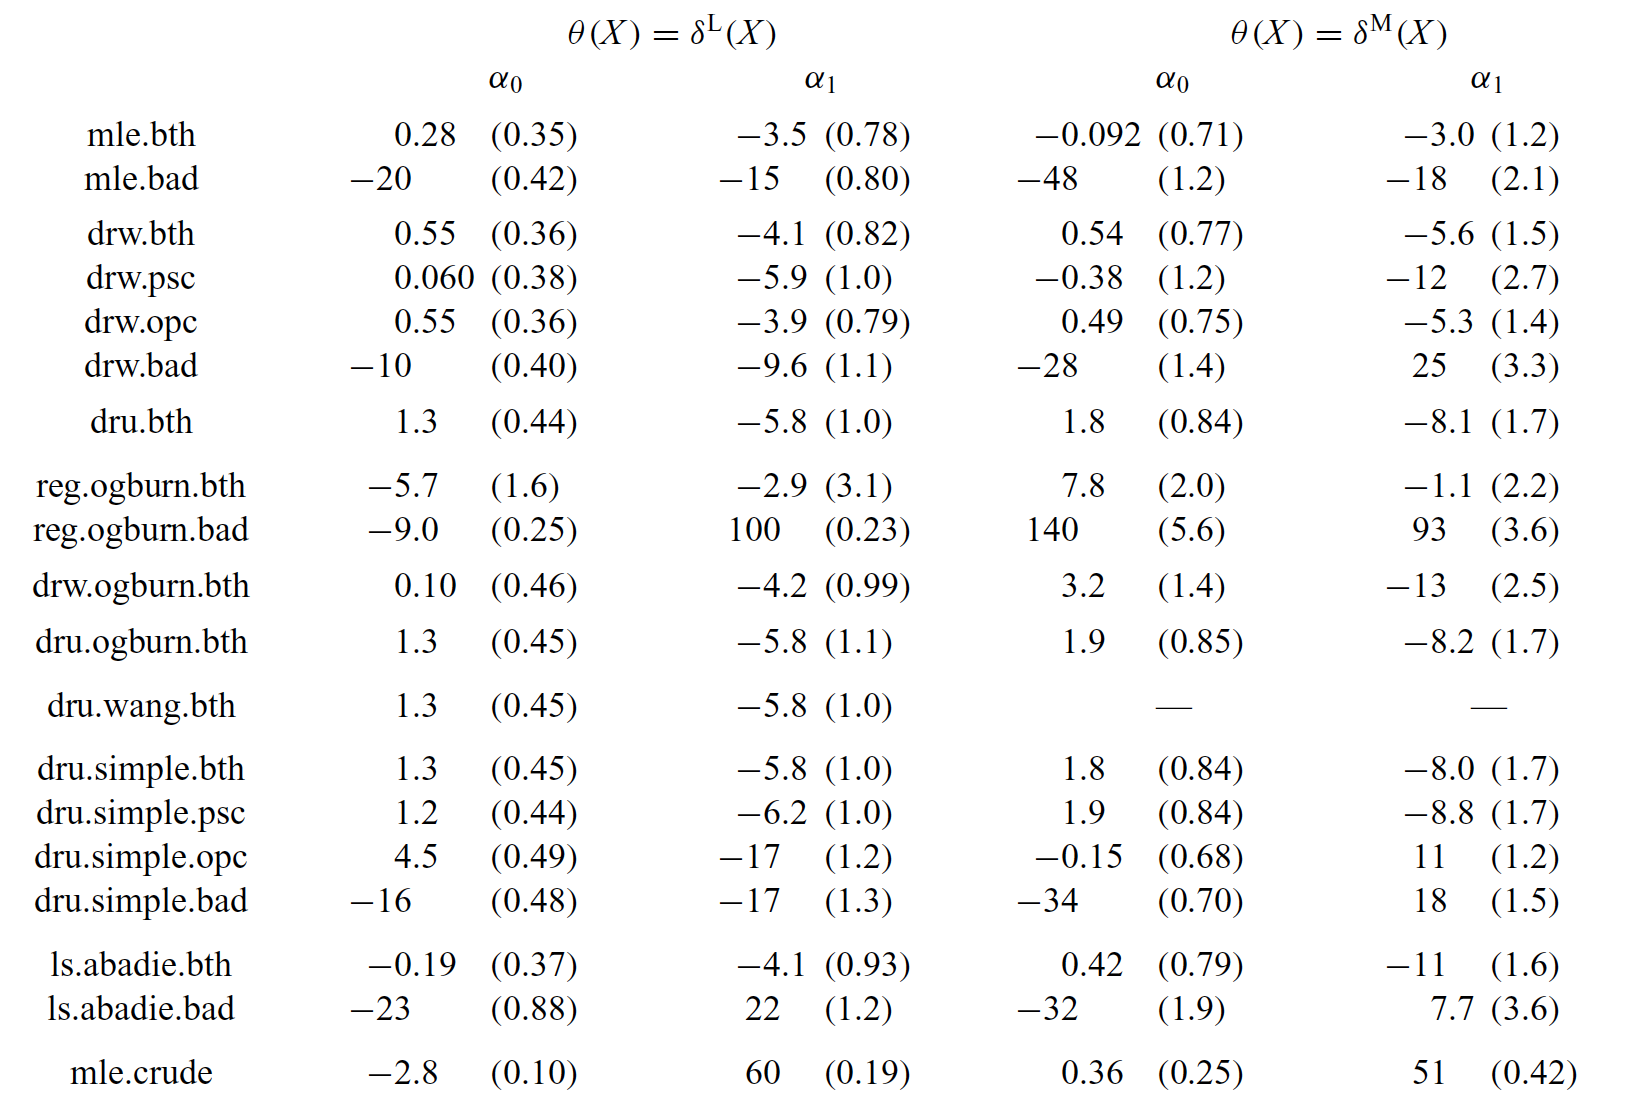
\includegraphics[width=0.65\textwidth]{figure/simulation.png}
\end{figure}
\end{frame}

\begin{frame}{401(k) Data}
The 401(k) plan has become the most popular employer-sponsored retirement plan in the U.S.A. Economists have long been interested in whether 401(k) contributions represent additional savings or simply replace other retirement plans, such as Individual Retirement Accounts.

Our 401(k) dataset contains 9275 individuals and the following variables:
\begin{itemize}
\item e401k                        =1 if eligble for 401(k).
\item inc                          annual income
\item marr                         =1 if married 
\item male                         =1 if male respondent 
\item age                          in years 
\item fsize                        family size  
\item nettfa                       net total fin. assets, 1000
\item p401k                        =1 if participate in 401(k) 
\item pira                         =1 if have IRA 
\end{itemize}
\end{frame}

\begin{frame}{401(k) Data}
We choose 
\begin{itemize}
\item e401(k) (eligble for 401(k)) as instrumental variable.
\item p401(k) (participation in 401(k)) as treatment indicator.
\item pira(k) (have IRA) as response variable.
\item intercept, inc, $inc^2$, age, marr, fsize as covariates.
\end{itemize}

Our model assumptions are:
\begin{itemize}
\item Local treatment effect is modelled as $\delta^M(X) = \exp(\alpha'X)$.
\item Since individuals may choose to participate in 401(k) plans, there are no defiers and or always takers. As a result, $\phi_2\equiv 0, \phi_2\phi_4=\equiv 0$, and the model of $P(D,Y|Z)$ can be determined by $\delta^M(X), \phi_1(X),\phi_3(X), OP^{CO}(X)$.
\end{itemize}
In our real data experiments, we use mle and drw without misspecification to estimate the parameters.
\end{frame}

\begin{frame}{401(k) Data: Results}
\begin{figure}
\begin{minipage}{0.4\textwidth}
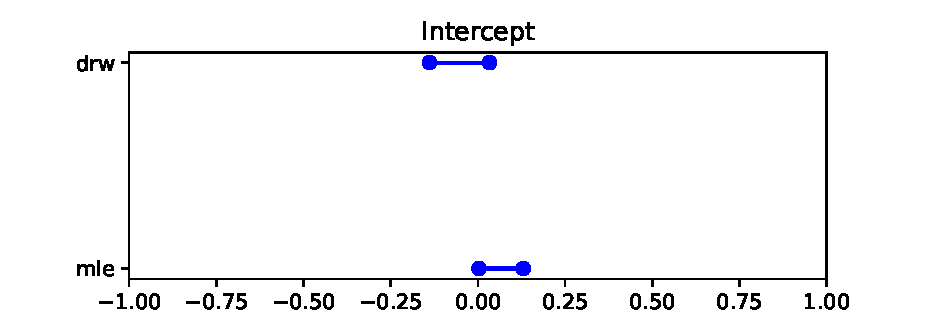
\includegraphics[width=\textwidth]{figure/0.eps}
\end{minipage}
\begin{minipage}{0.4\textwidth}
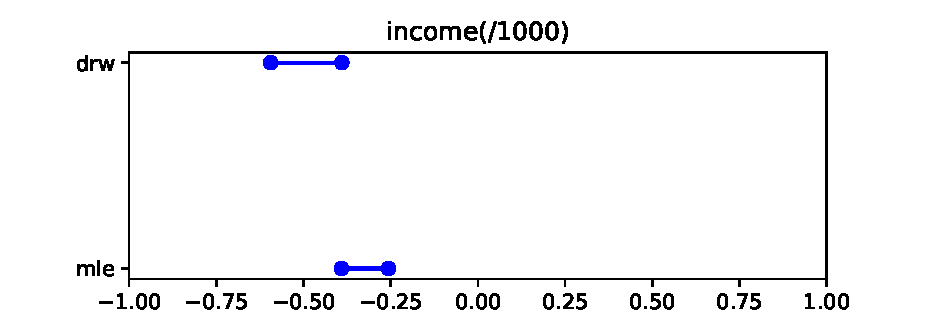
\includegraphics[width=\textwidth]{figure/1.eps}
\end{minipage}

\begin{minipage}{0.4\textwidth}
    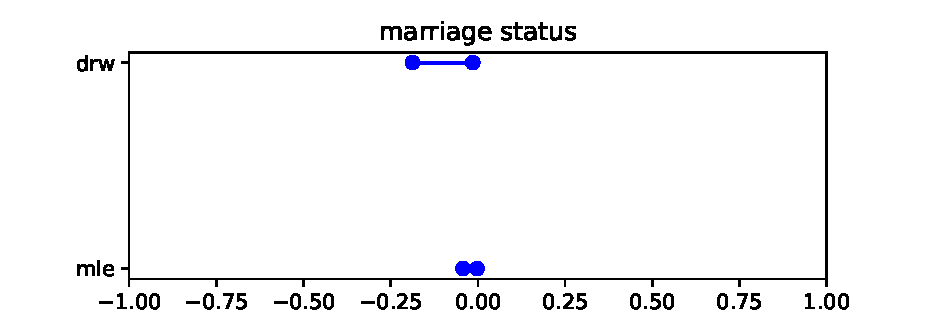
\includegraphics[width=\textwidth]{figure/2.eps}
    \end{minipage}
    \begin{minipage}{0.4\textwidth}
    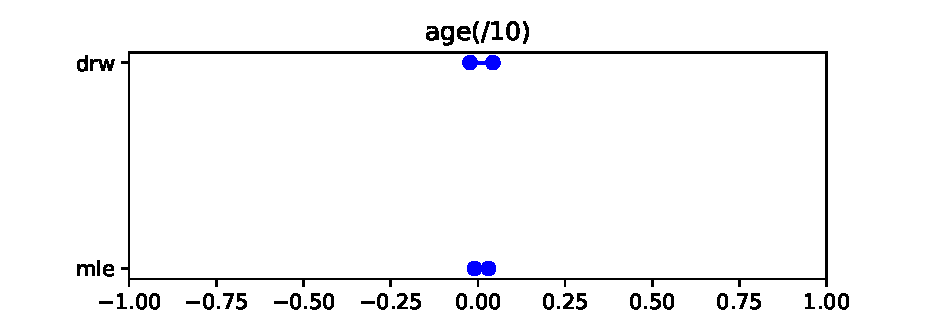
\includegraphics[width=\textwidth]{figure/3.eps}
    \end{minipage}

\begin{minipage}{0.4\textwidth}
    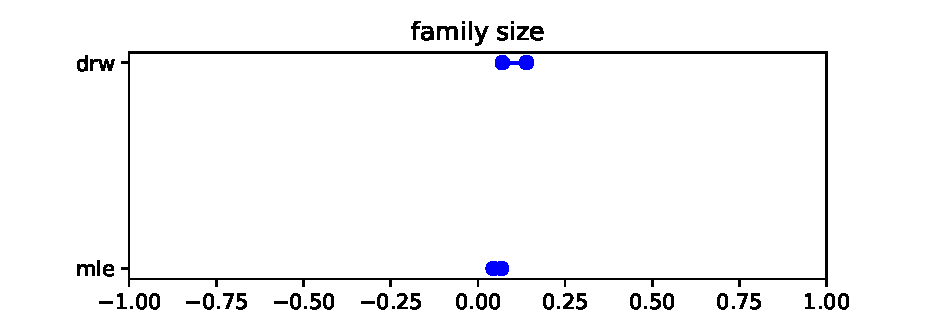
\includegraphics[width=\textwidth]{figure/4.eps}
    \end{minipage}
    \begin{minipage}{0.4\textwidth}
    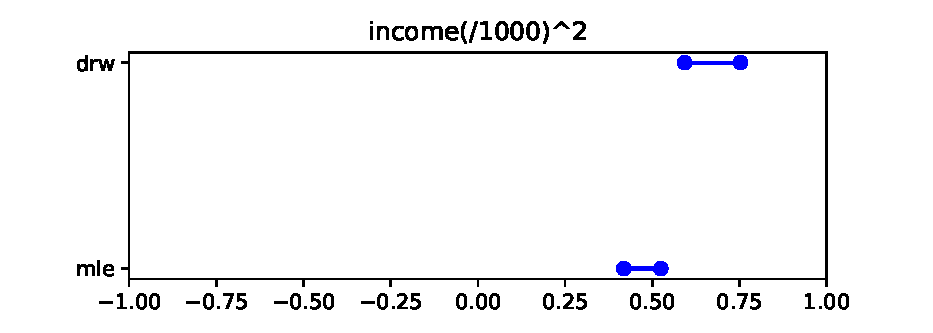
\includegraphics[width=\textwidth]{figure/5.eps}
    \end{minipage}
\caption{95\% confidence intervals of coefficients in MLATE using different methods}
\end{figure}
\end{frame}

\begin{frame}
Here are the results reported by the authors:
\begin{figure}
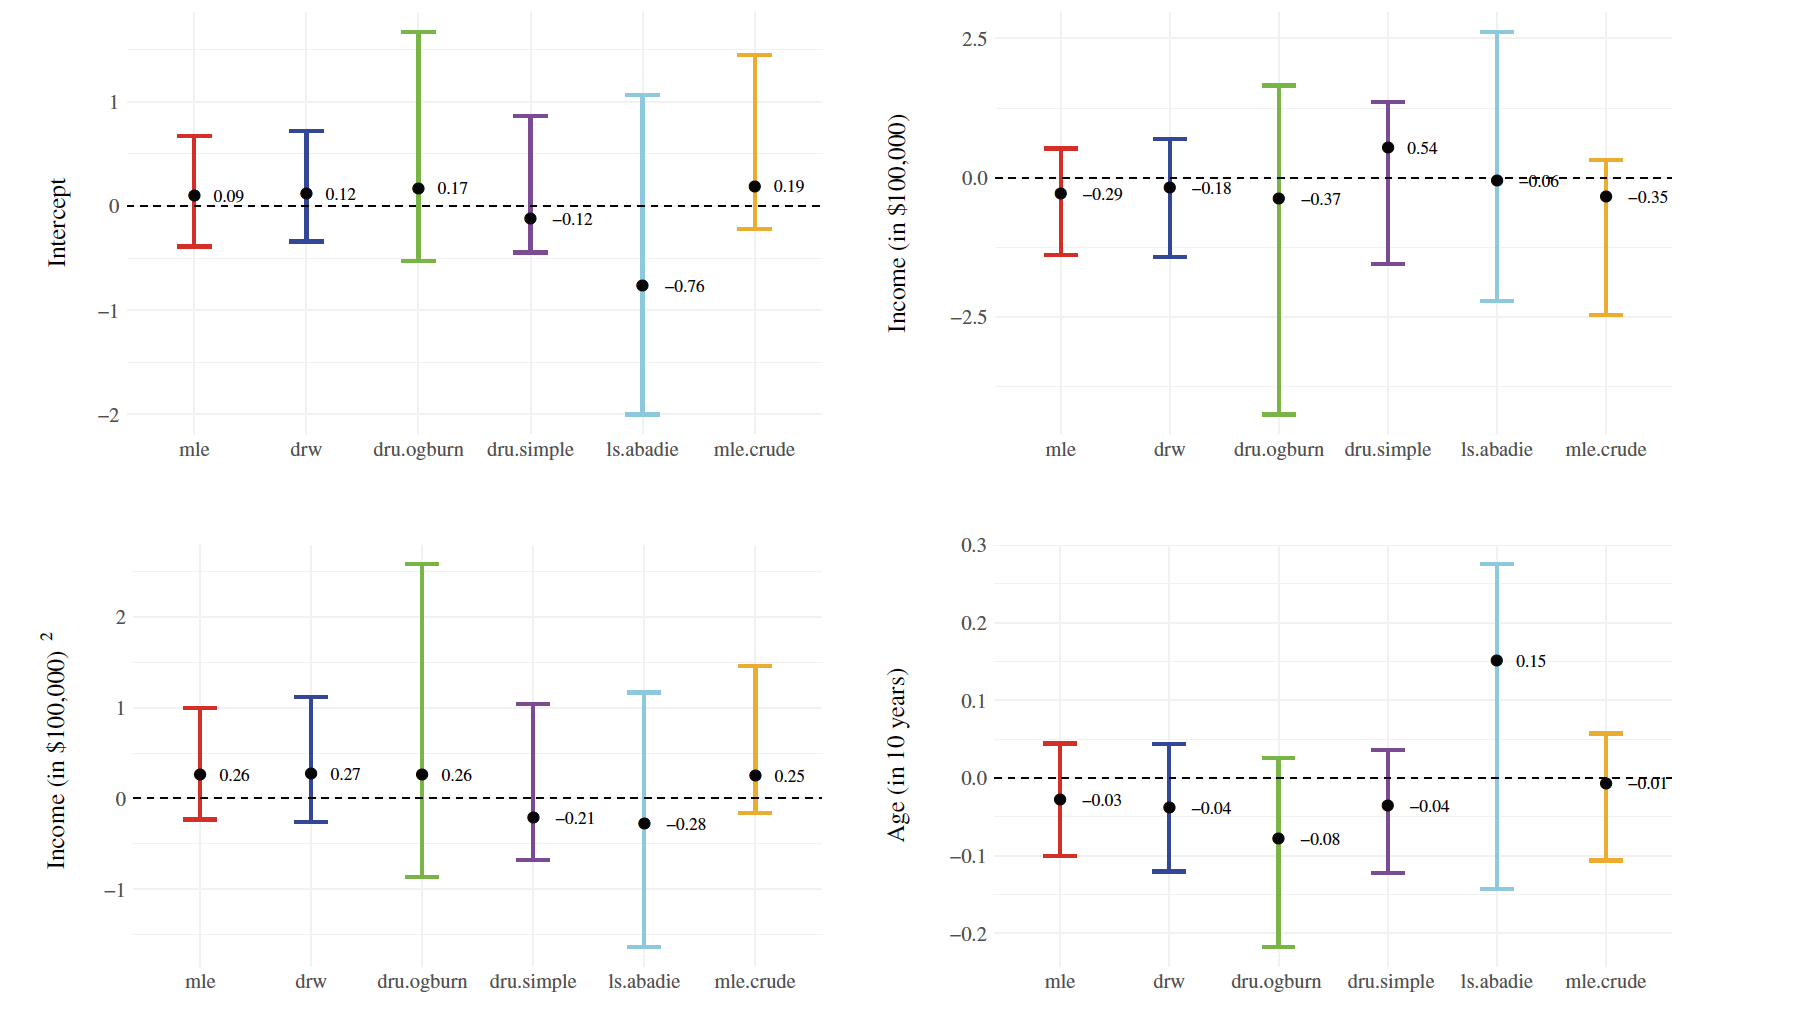
\includegraphics[width=0.8\textwidth]{figure/401k1.png}
\caption{95\% confidence intervals of coefficients in MLATE using different methods (Part I)}
\end{figure}
\end{frame}

\begin{frame}{401(k) Data: Results}
Here are the results reported by the authors:
\begin{figure}
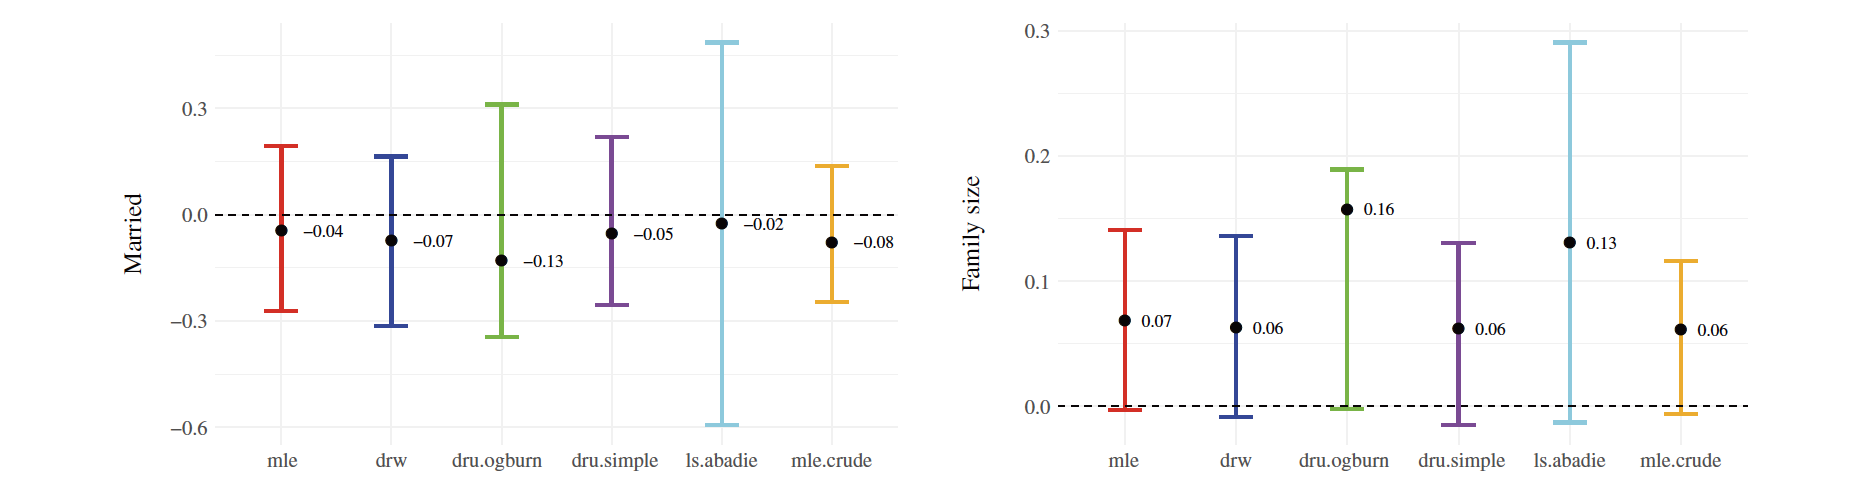
\includegraphics[width=0.9\textwidth]{figure/401k2.png}
\caption{95\% confidence intervals of coefficients in MLATE using different methods (Part II)}
\end{figure}
\end{frame}

\begin{frame}{401(k) Data: Results}
\begin{figure}
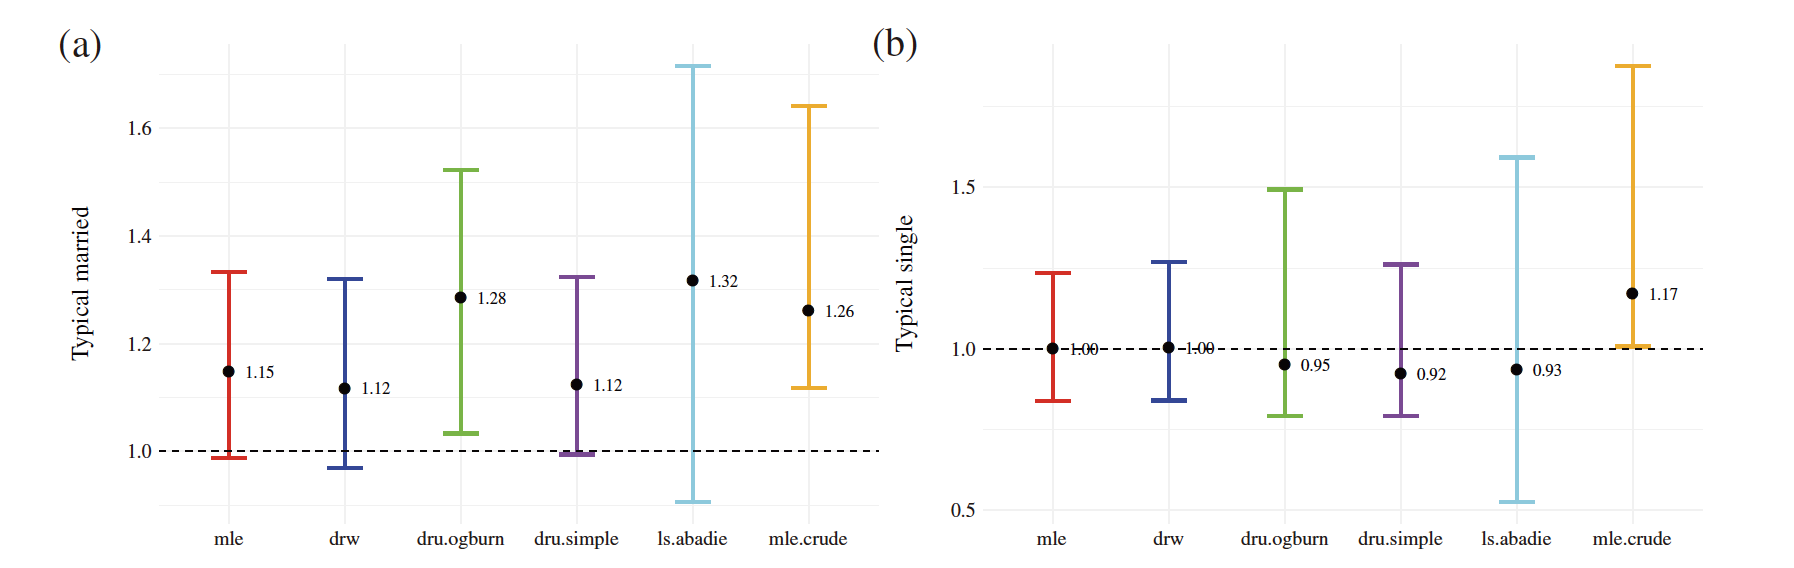
\includegraphics[width=0.9\textwidth]{figure/401k3.png}
\caption{95\% confidence intervals of MLATE using different methods}
\end{figure}
We may find that the two proposed methods (mle and drw) tend to give a conservative of local treatment effect and enjoy smaller variance.
\end{frame}
\end{document}